\documentclass[twoside]{book}

% Packages required by doxygen
\usepackage{fixltx2e}
\usepackage{calc}
\usepackage{doxygen}
\usepackage{graphicx}
\usepackage[utf8]{inputenc}
\usepackage{makeidx}
\usepackage{multicol}
\usepackage{multirow}
\PassOptionsToPackage{warn}{textcomp}
\usepackage{textcomp}
\usepackage[nointegrals]{wasysym}
\usepackage[table]{xcolor}

% Font selection
\usepackage[T1]{fontenc}
\usepackage{mathptmx}
\usepackage[scaled=.90]{helvet}
\usepackage{courier}
\usepackage{amssymb}
\usepackage{sectsty}
\renewcommand{\familydefault}{\sfdefault}
\allsectionsfont{%
  \fontseries{bc}\selectfont%
  \color{darkgray}%
}
\renewcommand{\DoxyLabelFont}{%
  \fontseries{bc}\selectfont%
  \color{darkgray}%
}
\newcommand{\+}{\discretionary{\mbox{\scriptsize$\hookleftarrow$}}{}{}}

% Page & text layout
\usepackage{geometry}
\geometry{%
  a4paper,%
  top=2.5cm,%
  bottom=2.5cm,%
  left=2.5cm,%
  right=2.5cm%
}
\tolerance=750
\hfuzz=15pt
\hbadness=750
\setlength{\emergencystretch}{15pt}
\setlength{\parindent}{0cm}
\setlength{\parskip}{0.2cm}
\makeatletter
\renewcommand{\paragraph}{%
  \@startsection{paragraph}{4}{0ex}{-1.0ex}{1.0ex}{%
    \normalfont\normalsize\bfseries\SS@parafont%
  }%
}
\renewcommand{\subparagraph}{%
  \@startsection{subparagraph}{5}{0ex}{-1.0ex}{1.0ex}{%
    \normalfont\normalsize\bfseries\SS@subparafont%
  }%
}
\makeatother

% Headers & footers
\usepackage{fancyhdr}
\pagestyle{fancyplain}
\fancyhead[LE]{\fancyplain{}{\bfseries\thepage}}
\fancyhead[CE]{\fancyplain{}{}}
\fancyhead[RE]{\fancyplain{}{\bfseries\leftmark}}
\fancyhead[LO]{\fancyplain{}{\bfseries\rightmark}}
\fancyhead[CO]{\fancyplain{}{}}
\fancyhead[RO]{\fancyplain{}{\bfseries\thepage}}
\fancyfoot[LE]{\fancyplain{}{}}
\fancyfoot[CE]{\fancyplain{}{}}
\fancyfoot[RE]{\fancyplain{}{\bfseries\scriptsize Generated on Wed Jun 28 2017 07\+:03\+:56 for C\+S\+I udp to server by Doxygen }}
\fancyfoot[LO]{\fancyplain{}{\bfseries\scriptsize Generated on Wed Jun 28 2017 07\+:03\+:56 for C\+S\+I udp to server by Doxygen }}
\fancyfoot[CO]{\fancyplain{}{}}
\fancyfoot[RO]{\fancyplain{}{}}
\renewcommand{\footrulewidth}{0.4pt}
\renewcommand{\chaptermark}[1]{%
  \markboth{#1}{}%
}
\renewcommand{\sectionmark}[1]{%
  \markright{\thesection\ #1}%
}

% Indices & bibliography
\usepackage{natbib}
\usepackage[titles]{tocloft}
\setcounter{tocdepth}{3}
\setcounter{secnumdepth}{5}
\makeindex

% Hyperlinks (required, but should be loaded last)
\usepackage{ifpdf}
\ifpdf
  \usepackage[pdftex,pagebackref=true]{hyperref}
\else
  \usepackage[ps2pdf,pagebackref=true]{hyperref}
\fi
\hypersetup{%
  colorlinks=true,%
  linkcolor=blue,%
  citecolor=blue,%
  unicode%
}

% Custom commands
\newcommand{\clearemptydoublepage}{%
  \newpage{\pagestyle{empty}\cleardoublepage}%
}


%===== C O N T E N T S =====

\begin{document}

% Titlepage & ToC
\hypersetup{pageanchor=false,
             bookmarks=true,
             bookmarksnumbered=true,
             pdfencoding=unicode
            }
\pagenumbering{roman}
\begin{titlepage}
\vspace*{7cm}
\begin{center}%
{\Large C\+S\+I udp to server \\[1ex]\large v1.\+0 }\\
\vspace*{1cm}
{\large Generated by Doxygen 1.8.8}\\
\vspace*{0.5cm}
{\small Wed Jun 28 2017 07:03:56}\\
\end{center}
\end{titlepage}
\clearemptydoublepage
\tableofcontents
\clearemptydoublepage
\pagenumbering{arabic}
\hypersetup{pageanchor=true}

%--- Begin generated contents ---
\chapter{Data Structure Index}
\section{Data Structures}
Here are the data structures with brief descriptions\+:\begin{DoxyCompactList}
\item\contentsline{section}{\hyperlink{structCOMPLEX}{C\+O\+M\+P\+L\+E\+X} }{\pageref{structCOMPLEX}}{}
\item\contentsline{section}{\hyperlink{structcsi__struct}{csi\+\_\+struct} }{\pageref{structcsi__struct}}{}
\end{DoxyCompactList}

\chapter{File Index}
\section{CSI liveview File List}
Here is a list of all files with brief descriptions:\begin{CompactList}
\item\contentsline{section}{{\bf \_\-\_\-init\_\-\_\-.py} }{\pageref{____init_____8py}}{}
\item\contentsline{section}{{\bf Atheros.py} }{\pageref{Atheros_8py}}{}
\item\contentsline{section}{{\bf Atheros\_\-plotandsave.py} }{\pageref{Atheros__plotandsave_8py}}{}
\item\contentsline{section}{{\bf Atheros\_\-readandplot\_\-in\_\-realtime.py} }{\pageref{Atheros__readandplot__in__realtime_8py}}{}
\item\contentsline{section}{{\bf docstring.py} }{\pageref{docstring_8py}}{}
\item\contentsline{section}{{\bf test.py} }{\pageref{test_8py}}{}
\item\contentsline{section}{{\bf udp.py} }{\pageref{udp_8py}}{}
\item\contentsline{section}{{\bf udp\_\-test.py} }{\pageref{udp__test_8py}}{}
\end{CompactList}

\chapter{Data Structure Documentation}
\hypertarget{structCOMPLEX}{\section{C\+O\+M\+P\+L\+E\+X Struct Reference}
\label{structCOMPLEX}\index{C\+O\+M\+P\+L\+E\+X@{C\+O\+M\+P\+L\+E\+X}}
}
\subsection*{Data Fields}
\begin{DoxyCompactItemize}
\item 
\hypertarget{structCOMPLEX_a102365412859377c432d9f5a0af670db}{int {\bfseries real}}\label{structCOMPLEX_a102365412859377c432d9f5a0af670db}

\item 
\hypertarget{structCOMPLEX_a794c97ac4d36c50108cb1de1345b7d5a}{int {\bfseries imag}}\label{structCOMPLEX_a794c97ac4d36c50108cb1de1345b7d5a}

\end{DoxyCompactItemize}


The documentation for this struct was generated from the following file\+:\begin{DoxyCompactItemize}
\item 
/home/shuspieler/\+Atheros-\/\+C\+S\+I-\/\+Tool-\/\+User\+Space-\/\+A\+P\+P/recv\+C\+S\+I-\/with-\/socket/\hyperlink{csi__fun_8h}{csi\+\_\+fun.\+h}\end{DoxyCompactItemize}

\hypertarget{structcsi__struct}{\section{csi\+\_\+struct Struct Reference}
\label{structcsi__struct}\index{csi\+\_\+struct@{csi\+\_\+struct}}
}
\subsection*{Data Fields}
\begin{DoxyCompactItemize}
\item 
\hypertarget{structcsi__struct_ac8ba20371dcdbdaeb85058f52ab3d868}{u\+\_\+int64\+\_\+t {\bfseries tstamp}}\label{structcsi__struct_ac8ba20371dcdbdaeb85058f52ab3d868}

\item 
\hypertarget{structcsi__struct_a61377724eca873f2240d9f783d2ba80b}{u\+\_\+int16\+\_\+t {\bfseries channel}}\label{structcsi__struct_a61377724eca873f2240d9f783d2ba80b}

\item 
\hypertarget{structcsi__struct_abbc6e4ea7e5715a804eb2dfd69cad603}{u\+\_\+int8\+\_\+t {\bfseries chan\+B\+W}}\label{structcsi__struct_abbc6e4ea7e5715a804eb2dfd69cad603}

\item 
\hypertarget{structcsi__struct_aaf5f341137b331e43bdbd8280f15d719}{u\+\_\+int8\+\_\+t {\bfseries rate}}\label{structcsi__struct_aaf5f341137b331e43bdbd8280f15d719}

\item 
\hypertarget{structcsi__struct_ad92ff4c838d8dc100865d28a0a802859}{u\+\_\+int8\+\_\+t {\bfseries nr}}\label{structcsi__struct_ad92ff4c838d8dc100865d28a0a802859}

\item 
\hypertarget{structcsi__struct_a7bc84a2f75977e4713d1ea09c1a9ca96}{u\+\_\+int8\+\_\+t {\bfseries nc}}\label{structcsi__struct_a7bc84a2f75977e4713d1ea09c1a9ca96}

\item 
\hypertarget{structcsi__struct_a553110c0bd159611593a51c3ae3fb2d2}{u\+\_\+int8\+\_\+t {\bfseries num\+\_\+tones}}\label{structcsi__struct_a553110c0bd159611593a51c3ae3fb2d2}

\item 
\hypertarget{structcsi__struct_acaa5ab531a3289b359b0af50478329ce}{u\+\_\+int8\+\_\+t {\bfseries noise}}\label{structcsi__struct_acaa5ab531a3289b359b0af50478329ce}

\item 
\hypertarget{structcsi__struct_aa6638fbb247fe3630300e4283e0f34f2}{u\+\_\+int8\+\_\+t {\bfseries phyerr}}\label{structcsi__struct_aa6638fbb247fe3630300e4283e0f34f2}

\item 
\hypertarget{structcsi__struct_a81517650e0bd4b40b69cbb7519862ad9}{u\+\_\+int8\+\_\+t {\bfseries rssi}}\label{structcsi__struct_a81517650e0bd4b40b69cbb7519862ad9}

\item 
\hypertarget{structcsi__struct_abe7e5ea18326e92122ecf1e6cce77355}{u\+\_\+int8\+\_\+t {\bfseries rssi\+\_\+0}}\label{structcsi__struct_abe7e5ea18326e92122ecf1e6cce77355}

\item 
\hypertarget{structcsi__struct_afca064b2c4623ad1d55d56063bb4c78a}{u\+\_\+int8\+\_\+t {\bfseries rssi\+\_\+1}}\label{structcsi__struct_afca064b2c4623ad1d55d56063bb4c78a}

\item 
\hypertarget{structcsi__struct_a063f3e3d0def7a2dab87c850fdcca617}{u\+\_\+int8\+\_\+t {\bfseries rssi\+\_\+2}}\label{structcsi__struct_a063f3e3d0def7a2dab87c850fdcca617}

\item 
\hypertarget{structcsi__struct_a720918e326e84706700c4fa610ec2450}{u\+\_\+int16\+\_\+t {\bfseries payload\+\_\+len}}\label{structcsi__struct_a720918e326e84706700c4fa610ec2450}

\item 
\hypertarget{structcsi__struct_ae81d4b882c49c003ed821d6ccbb970b6}{u\+\_\+int16\+\_\+t {\bfseries csi\+\_\+len}}\label{structcsi__struct_ae81d4b882c49c003ed821d6ccbb970b6}

\item 
\hypertarget{structcsi__struct_a4d1117d5f7f471c95f78273a5ecc8d50}{u\+\_\+int16\+\_\+t {\bfseries buf\+\_\+len}}\label{structcsi__struct_a4d1117d5f7f471c95f78273a5ecc8d50}

\end{DoxyCompactItemize}


The documentation for this struct was generated from the following file\+:\begin{DoxyCompactItemize}
\item 
/home/shuspieler/\+Atheros-\/\+C\+S\+I-\/\+Tool-\/\+User\+Space-\/\+A\+P\+P/recv\+C\+S\+I-\/with-\/socket/\hyperlink{csi__fun_8h}{csi\+\_\+fun.\+h}\end{DoxyCompactItemize}

\chapter{File Documentation}
\hypertarget{csi__fun_8c}{\section{/home/shuspieler/\+Atheros-\/\+C\+S\+I-\/\+Tool-\/\+User\+Space-\/\+A\+P\+P/recv\+C\+S\+I-\/with-\/socket/csi\+\_\+fun.c File Reference}
\label{csi__fun_8c}\index{/home/shuspieler/\+Atheros-\/\+C\+S\+I-\/\+Tool-\/\+User\+Space-\/\+A\+P\+P/recv\+C\+S\+I-\/with-\/socket/csi\+\_\+fun.\+c@{/home/shuspieler/\+Atheros-\/\+C\+S\+I-\/\+Tool-\/\+User\+Space-\/\+A\+P\+P/recv\+C\+S\+I-\/with-\/socket/csi\+\_\+fun.\+c}}
}


basic csi processing fucntion  


{\ttfamily \#include $<$stdlib.\+h$>$}\\*
{\ttfamily \#include $<$stdio.\+h$>$}\\*
{\ttfamily \#include $<$stdbool.\+h$>$}\\*
{\ttfamily \#include $<$string.\+h$>$}\\*
{\ttfamily \#include $<$unistd.\+h$>$}\\*
{\ttfamily \#include $<$fcntl.\+h$>$}\\*
{\ttfamily \#include \char`\"{}csi\+\_\+fun.\+h\char`\"{}}\\*
Include dependency graph for csi\+\_\+fun.\+c\+:\nopagebreak
\begin{figure}[H]
\begin{center}
\leavevmode
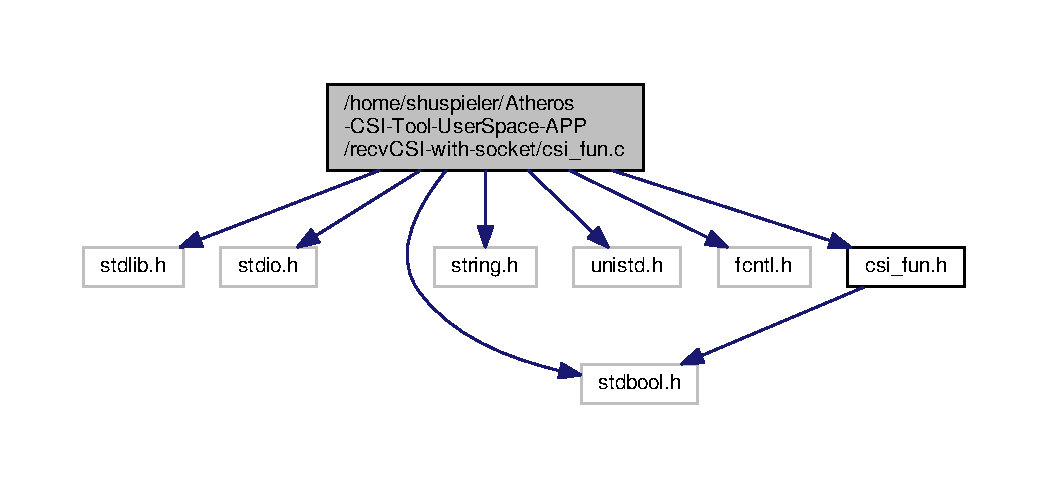
\includegraphics[width=350pt]{csi__fun_8c__incl}
\end{center}
\end{figure}
\subsection*{Macros}
\begin{DoxyCompactItemize}
\item 
\hypertarget{csi__fun_8c_a4918568b8b7021b777ae00bd7be2fc14}{\#define {\bfseries csi\+\_\+st\+\_\+len}~23}\label{csi__fun_8c_a4918568b8b7021b777ae00bd7be2fc14}

\end{DoxyCompactItemize}
\subsection*{Functions}
\begin{DoxyCompactItemize}
\item 
\hypertarget{csi__fun_8c_aed5f3e73e01248d8a2d6792a69081f9e}{bool {\bfseries is\+\_\+big\+\_\+endian} ()}\label{csi__fun_8c_aed5f3e73e01248d8a2d6792a69081f9e}

\item 
\hypertarget{csi__fun_8c_a501a25d41e6e80a5bfcf1dd375a16bd7}{int {\bfseries bit\+\_\+convert} (int data, int maxbit)}\label{csi__fun_8c_a501a25d41e6e80a5bfcf1dd375a16bd7}

\item 
\hypertarget{csi__fun_8c_afd68310d3f1cb2aca7abb7da551195d0}{void {\bfseries fill\+\_\+csi\+\_\+matrix} (u\+\_\+int8\+\_\+t $\ast$csi\+\_\+addr, int nr, int nc, int num\+\_\+tones, \hyperlink{structCOMPLEX}{C\+O\+M\+P\+L\+E\+X}($\ast$csi\+\_\+matrix)\mbox{[}3\mbox{]}\mbox{[}114\mbox{]})}\label{csi__fun_8c_afd68310d3f1cb2aca7abb7da551195d0}

\item 
\hypertarget{csi__fun_8c_a99fac622f5ac7ca70c01b972b07b93cf}{int {\bfseries open\+\_\+csi\+\_\+device} ()}\label{csi__fun_8c_a99fac622f5ac7ca70c01b972b07b93cf}

\item 
\hypertarget{csi__fun_8c_a207679327e5eaea46de448f0bb80ca86}{void {\bfseries close\+\_\+csi\+\_\+device} (int fd)}\label{csi__fun_8c_a207679327e5eaea46de448f0bb80ca86}

\item 
\hypertarget{csi__fun_8c_aa3bb68539af1843371ac0554235dffae}{int {\bfseries read\+\_\+csi\+\_\+buf} (unsigned char $\ast$buf\+\_\+addr, int fd, int B\+U\+F\+S\+I\+Z\+E)}\label{csi__fun_8c_aa3bb68539af1843371ac0554235dffae}

\item 
\hypertarget{csi__fun_8c_a40a1ee251b887facc992e28711ebd8b6}{void {\bfseries record\+\_\+status} (unsigned char $\ast$buf\+\_\+addr, int cnt, \hyperlink{structcsi__struct}{csi\+\_\+struct} $\ast$csi\+\_\+status)}\label{csi__fun_8c_a40a1ee251b887facc992e28711ebd8b6}

\item 
\hypertarget{csi__fun_8c_ad0936a891497fb3413bc12df35a92b15}{void {\bfseries record\+\_\+csi\+\_\+payload} (unsigned char $\ast$buf\+\_\+addr, \hyperlink{structcsi__struct}{csi\+\_\+struct} $\ast$csi\+\_\+status, unsigned char $\ast$data\+\_\+buf, \hyperlink{structCOMPLEX}{C\+O\+M\+P\+L\+E\+X}($\ast$csi\+\_\+matrix)\mbox{[}3\mbox{]}\mbox{[}114\mbox{]})}\label{csi__fun_8c_ad0936a891497fb3413bc12df35a92b15}

\item 
\hypertarget{csi__fun_8c_afa9350afae7ab5a1eac665b050736fc0}{void {\bfseries porcess\+\_\+csi} (unsigned char $\ast$data\+\_\+buf, \hyperlink{structcsi__struct}{csi\+\_\+struct} $\ast$csi\+\_\+status, \hyperlink{structCOMPLEX}{C\+O\+M\+P\+L\+E\+X}($\ast$csi\+\_\+buf)\mbox{[}3\mbox{]}\mbox{[}114\mbox{]})}\label{csi__fun_8c_afa9350afae7ab5a1eac665b050736fc0}

\end{DoxyCompactItemize}


\subsection{Detailed Description}
basic csi processing fucntion 

=====================================================================================

you can implement your own fucntion here

\begin{DoxyVersion}{Version}
\+: 1.\+0
\end{DoxyVersion}
\begin{DoxyAuthor}{Author}
\+: Yaxiong Xie
\end{DoxyAuthor}
Email \+: \href{mailto:xieyaxiongfly@gmail.com}{\tt xieyaxiongfly@gmail.\+com}

Organization\+: W\+A\+N\+D\+S group @ Nanyang Technological University

Copyright (c) W\+A\+N\+D\+S group @ Nanyang Technological University 


\hypertarget{csi__fun_8h}{\section{/home/shuspieler/\+Atheros-\/\+C\+S\+I-\/\+Tool-\/\+User\+Space-\/\+A\+P\+P/recv\+C\+S\+I-\/with-\/socket/csi\+\_\+fun.h File Reference}
\label{csi__fun_8h}\index{/home/shuspieler/\+Atheros-\/\+C\+S\+I-\/\+Tool-\/\+User\+Space-\/\+A\+P\+P/recv\+C\+S\+I-\/with-\/socket/csi\+\_\+fun.\+h@{/home/shuspieler/\+Atheros-\/\+C\+S\+I-\/\+Tool-\/\+User\+Space-\/\+A\+P\+P/recv\+C\+S\+I-\/with-\/socket/csi\+\_\+fun.\+h}}
}


head file for csi processing fucntion  


{\ttfamily \#include $<$stdbool.\+h$>$}\\*
Include dependency graph for csi\+\_\+fun.\+h\+:\nopagebreak
\begin{figure}[H]
\begin{center}
\leavevmode
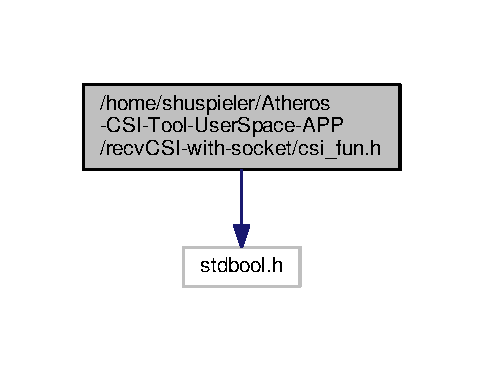
\includegraphics[width=232pt]{csi__fun_8h__incl}
\end{center}
\end{figure}
This graph shows which files directly or indirectly include this file\+:\nopagebreak
\begin{figure}[H]
\begin{center}
\leavevmode
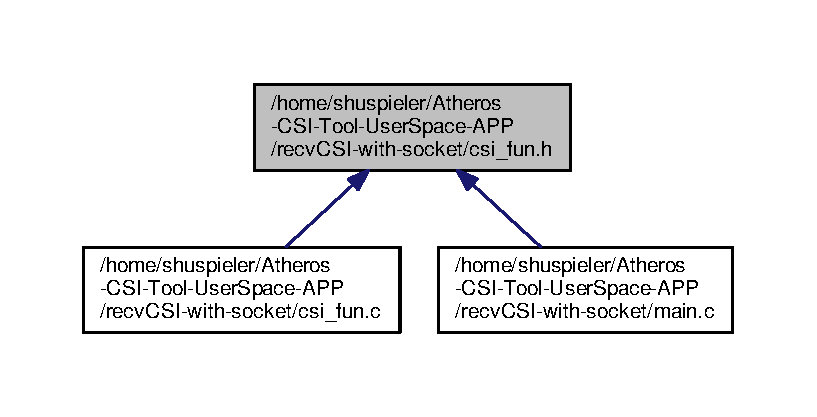
\includegraphics[width=350pt]{csi__fun_8h__dep__incl}
\end{center}
\end{figure}
\subsection*{Data Structures}
\begin{DoxyCompactItemize}
\item 
struct \hyperlink{structCOMPLEX}{C\+O\+M\+P\+L\+E\+X}
\item 
struct \hyperlink{structcsi__struct}{csi\+\_\+struct}
\end{DoxyCompactItemize}
\subsection*{Macros}
\begin{DoxyCompactItemize}
\item 
\hypertarget{csi__fun_8h_a389034e92c00d57ac17143a2db0cff54}{\#define {\bfseries Kernel\+\_\+\+C\+S\+I\+\_\+\+S\+T\+\_\+\+L\+E\+N}~23}\label{csi__fun_8h_a389034e92c00d57ac17143a2db0cff54}

\end{DoxyCompactItemize}
\subsection*{Functions}
\begin{DoxyCompactItemize}
\item 
\hypertarget{csi__fun_8h_aed5f3e73e01248d8a2d6792a69081f9e}{bool {\bfseries is\+\_\+big\+\_\+endian} ()}\label{csi__fun_8h_aed5f3e73e01248d8a2d6792a69081f9e}

\item 
\hypertarget{csi__fun_8h_a99fac622f5ac7ca70c01b972b07b93cf}{int {\bfseries open\+\_\+csi\+\_\+device} ()}\label{csi__fun_8h_a99fac622f5ac7ca70c01b972b07b93cf}

\item 
\hypertarget{csi__fun_8h_a207679327e5eaea46de448f0bb80ca86}{void {\bfseries close\+\_\+csi\+\_\+device} (int fd)}\label{csi__fun_8h_a207679327e5eaea46de448f0bb80ca86}

\item 
\hypertarget{csi__fun_8h_aa3bb68539af1843371ac0554235dffae}{int {\bfseries read\+\_\+csi\+\_\+buf} (unsigned char $\ast$buf\+\_\+addr, int fd, int B\+U\+F\+S\+I\+Z\+E)}\label{csi__fun_8h_aa3bb68539af1843371ac0554235dffae}

\item 
\hypertarget{csi__fun_8h_a40a1ee251b887facc992e28711ebd8b6}{void {\bfseries record\+\_\+status} (unsigned char $\ast$buf\+\_\+addr, int cnt, \hyperlink{structcsi__struct}{csi\+\_\+struct} $\ast$csi\+\_\+status)}\label{csi__fun_8h_a40a1ee251b887facc992e28711ebd8b6}

\item 
\hypertarget{csi__fun_8h_a40e91176bbd23b1a1a611cce733314c0}{void {\bfseries record\+\_\+csi\+\_\+payload} (unsigned char $\ast$buf\+\_\+addr, \hyperlink{structcsi__struct}{csi\+\_\+struct} $\ast$csi\+\_\+status, unsigned char $\ast$data\+\_\+buf, \hyperlink{structCOMPLEX}{C\+O\+M\+P\+L\+E\+X}($\ast$csi\+\_\+buf)\mbox{[}3\mbox{]}\mbox{[}114\mbox{]})}\label{csi__fun_8h_a40e91176bbd23b1a1a611cce733314c0}

\item 
\hypertarget{csi__fun_8h_afa9350afae7ab5a1eac665b050736fc0}{void {\bfseries porcess\+\_\+csi} (unsigned char $\ast$data\+\_\+buf, \hyperlink{structcsi__struct}{csi\+\_\+struct} $\ast$csi\+\_\+status, \hyperlink{structCOMPLEX}{C\+O\+M\+P\+L\+E\+X}($\ast$csi\+\_\+buf)\mbox{[}3\mbox{]}\mbox{[}114\mbox{]})}\label{csi__fun_8h_afa9350afae7ab5a1eac665b050736fc0}

\end{DoxyCompactItemize}


\subsection{Detailed Description}
head file for csi processing fucntion 

=====================================================================================

\begin{DoxyVersion}{Version}
\+: 1.\+0
\end{DoxyVersion}
\begin{DoxyAuthor}{Author}
\+: Yaxiong Xie
\end{DoxyAuthor}
Email \+: \href{mailto:xieyaxiongfly@gmail.com}{\tt xieyaxiongfly@gmail.\+com}

Organization\+: W\+A\+N\+D\+S group @ Nanyang Technological University

Copyright (c) W\+A\+N\+D\+S group @ Nanyang Technological University 


\hypertarget{main_8c}{\section{/home/shuspieler/\+Atheros-\/\+C\+S\+I-\/\+Tool-\/\+User\+Space-\/\+A\+P\+P/recv\+C\+S\+I-\/with-\/socket/main.c File Reference}
\label{main_8c}\index{/home/shuspieler/\+Atheros-\/\+C\+S\+I-\/\+Tool-\/\+User\+Space-\/\+A\+P\+P/recv\+C\+S\+I-\/with-\/socket/main.\+c@{/home/shuspieler/\+Atheros-\/\+C\+S\+I-\/\+Tool-\/\+User\+Space-\/\+A\+P\+P/recv\+C\+S\+I-\/with-\/socket/main.\+c}}
}


main function\+: log C\+S\+I to file or to server or to both.  


{\ttfamily \#include $<$stdlib.\+h$>$}\\*
{\ttfamily \#include $<$stdio.\+h$>$}\\*
{\ttfamily \#include $<$string.\+h$>$}\\*
{\ttfamily \#include $<$unistd.\+h$>$}\\*
{\ttfamily \#include $<$fcntl.\+h$>$}\\*
{\ttfamily \#include $<$errno.\+h$>$}\\*
{\ttfamily \#include $<$termios.\+h$>$}\\*
{\ttfamily \#include $<$pthread.\+h$>$}\\*
{\ttfamily \#include $<$signal.\+h$>$}\\*
{\ttfamily \#include $<$sys/types.\+h$>$}\\*
{\ttfamily \#include $<$sys/stat.\+h$>$}\\*
{\ttfamily \#include \char`\"{}csi\+\_\+fun.\+h\char`\"{}}\\*
{\ttfamily \#include \char`\"{}udp.\+c\char`\"{}}\\*
Include dependency graph for main.\+c\+:\nopagebreak
\begin{figure}[H]
\begin{center}
\leavevmode
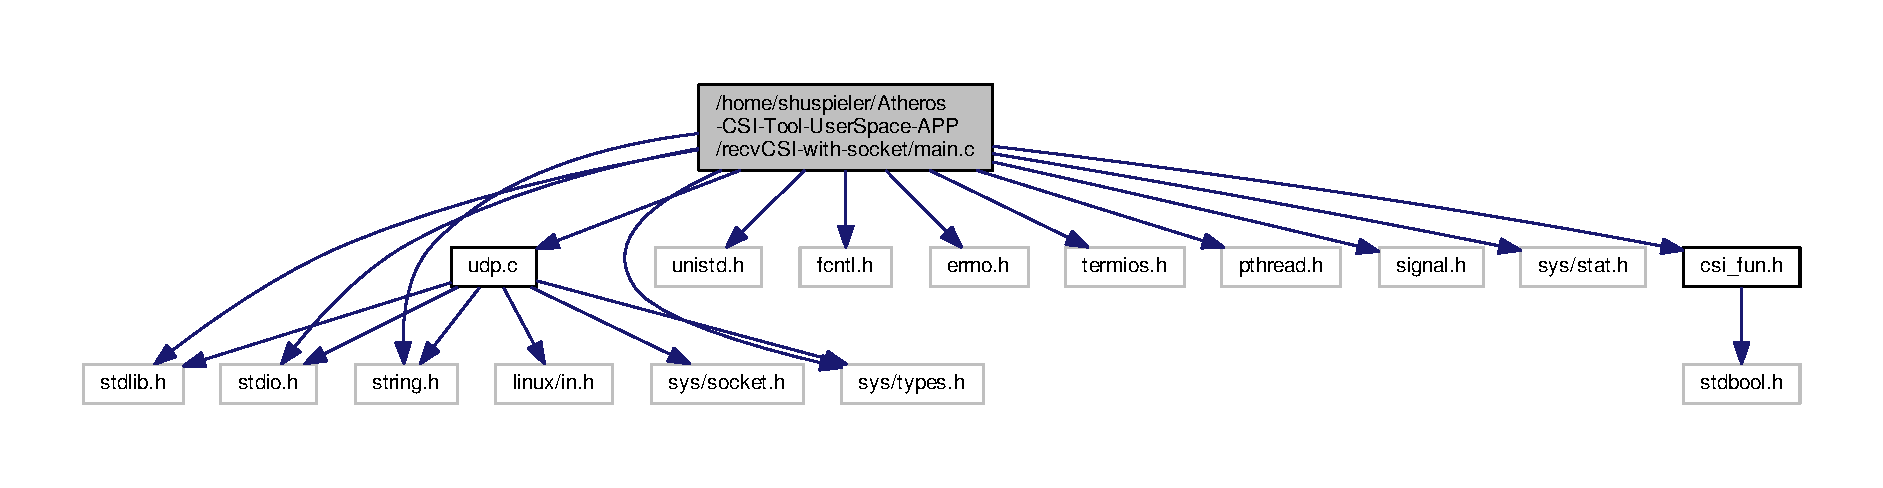
\includegraphics[width=350pt]{main_8c__incl}
\end{center}
\end{figure}
\subsection*{Macros}
\begin{DoxyCompactItemize}
\item 
\hypertarget{main_8c_aeca034f67218340ecb2261a22c2f3dcd}{\#define {\bfseries B\+U\+F\+S\+I\+Z\+E}~4096}\label{main_8c_aeca034f67218340ecb2261a22c2f3dcd}

\end{DoxyCompactItemize}
\subsection*{Functions}
\begin{DoxyCompactItemize}
\item 
\hypertarget{main_8c_a4f31a6fd48ee5d4579ae4aaaa3cae285}{void {\bfseries sig\+\_\+handler} (int signo)}\label{main_8c_a4f31a6fd48ee5d4579ae4aaaa3cae285}

\item 
int \hyperlink{main_8c_a0ddf1224851353fc92bfbff6f499fa97}{main} (int argc, char $\ast$argv\mbox{[}$\,$\mbox{]})
\end{DoxyCompactItemize}
\subsection*{Variables}
\begin{DoxyCompactItemize}
\item 
\hypertarget{main_8c_a2896431d6a80cd39b3d24b40237612ee}{int {\bfseries quit}}\label{main_8c_a2896431d6a80cd39b3d24b40237612ee}

\item 
\hypertarget{main_8c_a9f58335fad30c6bd2b698625a3d73d69}{unsigned char {\bfseries buf\+\_\+addr} \mbox{[}B\+U\+F\+S\+I\+Z\+E\mbox{]}}\label{main_8c_a9f58335fad30c6bd2b698625a3d73d69}

\item 
\hypertarget{main_8c_a063bbc9223e9af84c5c89bac0fe07c97}{unsigned char {\bfseries data\+\_\+buf} \mbox{[}1500\mbox{]}}\label{main_8c_a063bbc9223e9af84c5c89bac0fe07c97}

\item 
\hypertarget{main_8c_a436cda53ccd071f63670e70d88352a89}{\hyperlink{structCOMPLEX}{C\+O\+M\+P\+L\+E\+X} {\bfseries csi\+\_\+matrix} \mbox{[}3\mbox{]}\mbox{[}3\mbox{]}\mbox{[}114\mbox{]}}\label{main_8c_a436cda53ccd071f63670e70d88352a89}

\item 
\hypertarget{main_8c_a7d2f33c074a1b238be658ca6a049110c}{\hyperlink{structcsi__struct}{csi\+\_\+struct} $\ast$ {\bfseries csi\+\_\+status}}\label{main_8c_a7d2f33c074a1b238be658ca6a049110c}

\end{DoxyCompactItemize}


\subsection{Detailed Description}
main function\+: log C\+S\+I to file or to server or to both. 

=====================================================================================

Here is an example for receiving C\+S\+I matrix, Basic C\+Si procesing fucntion is also implemented and called, Check \hyperlink{csi__fun_8c}{csi\+\_\+fun.\+c} for detail of the processing function;

A function which log the C\+S\+I to a server is added in.

\begin{DoxyVersion}{Version}
\+: 2.\+0
\end{DoxyVersion}
\begin{DoxyAuthor}{Author}
\+: Yaxiong Xie
\end{DoxyAuthor}
modified by\+: Shu Ren

Email \+: \href{mailto:xieyaxiongfly@gmail.com}{\tt xieyaxiongfly@gmail.\+com}; \href{mailto:ierenshu@163.com}{\tt ierenshu@163.\+com}

Organization\+: W\+A\+N\+D\+S group @ Nanyang Technological University; L\+I\+K\+E @ F\+A\+U

Copyright (c) W\+A\+N\+D\+S group @ Nanyang Technological University; L\+I\+K\+E @ F\+A\+U 



\subsection{Function Documentation}
\hypertarget{main_8c_a0ddf1224851353fc92bfbff6f499fa97}{\index{main.\+c@{main.\+c}!main@{main}}
\index{main@{main}!main.\+c@{main.\+c}}
\subsubsection[{main}]{\setlength{\rightskip}{0pt plus 5cm}int main (
\begin{DoxyParamCaption}
\item[{int}]{argc, }
\item[{char $\ast$}]{argv\mbox{[}$\,$\mbox{]}}
\end{DoxyParamCaption}
)}}\label{main_8c_a0ddf1224851353fc92bfbff6f499fa97}
receive C\+S\+I and save to a file or send to a server or both

Usage 1\+: recv\+\_\+csi $<$output\+\_\+file$>$

Usage 2\+: recv\+\_\+csi $<$Server-\/ip$>$ $<$port$>$

Usage 3\+: recv\+\_\+csi $<$ip$>$ $<$port$>$ $<$output\+\_\+file$>$ 
\hypertarget{udp_8c}{\section{/home/shuspieler/\+Atheros-\/\+C\+S\+I-\/\+Tool-\/\+User\+Space-\/\+A\+P\+P/recv\+C\+S\+I-\/with-\/socket/udp.c File Reference}
\label{udp_8c}\index{/home/shuspieler/\+Atheros-\/\+C\+S\+I-\/\+Tool-\/\+User\+Space-\/\+A\+P\+P/recv\+C\+S\+I-\/with-\/socket/udp.\+c@{/home/shuspieler/\+Atheros-\/\+C\+S\+I-\/\+Tool-\/\+User\+Space-\/\+A\+P\+P/recv\+C\+S\+I-\/with-\/socket/udp.\+c}}
}


init and close function for socket(udp)  


{\ttfamily \#include $<$stdio.\+h$>$}\\*
{\ttfamily \#include $<$stdlib.\+h$>$}\\*
{\ttfamily \#include $<$string.\+h$>$}\\*
{\ttfamily \#include $<$sys/types.\+h$>$}\\*
{\ttfamily \#include $<$sys/socket.\+h$>$}\\*
{\ttfamily \#include $<$linux/in.\+h$>$}\\*
Include dependency graph for udp.\+c\+:\nopagebreak
\begin{figure}[H]
\begin{center}
\leavevmode
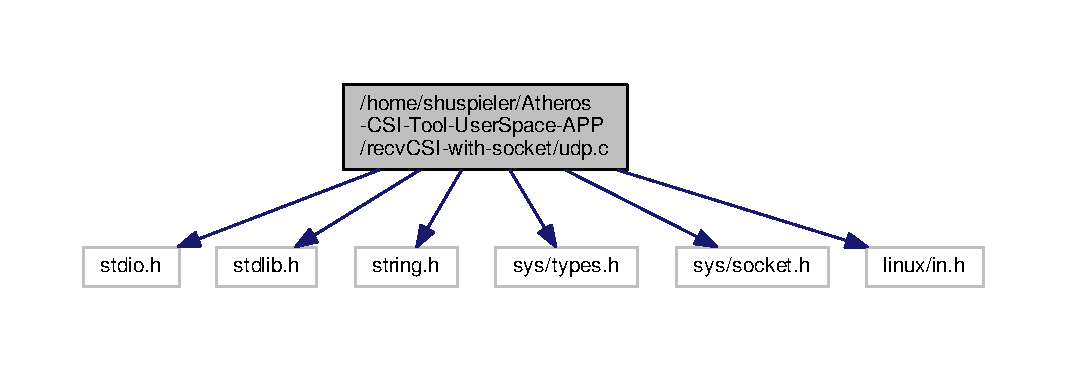
\includegraphics[width=350pt]{udp_8c__incl}
\end{center}
\end{figure}
This graph shows which files directly or indirectly include this file\+:\nopagebreak
\begin{figure}[H]
\begin{center}
\leavevmode
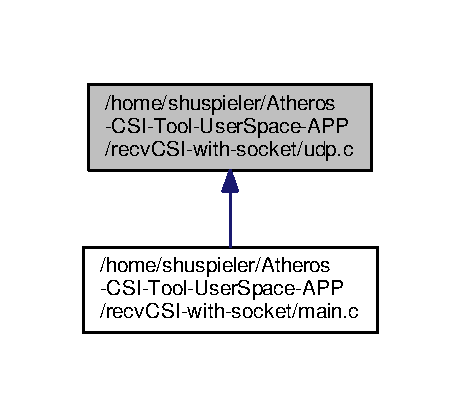
\includegraphics[width=221pt]{udp_8c__dep__incl}
\end{center}
\end{figure}
\subsection*{Functions}
\begin{DoxyCompactItemize}
\item 
int \hyperlink{udp_8c_aff119789f658dc4654c7d31d04caa9ea}{init\+\_\+udp} (const char $\ast$strptr, unsigned short portnum)
\item 
int \hyperlink{udp_8c_a7e1d80b405a569a1d308aa0b9244514d}{close\+\_\+udp} (int cfd)
\end{DoxyCompactItemize}


\subsection{Detailed Description}
init and close function for socket(udp) 

=====================================================================================

\begin{DoxyVersion}{Version}
1.\+0
\end{DoxyVersion}
\begin{DoxyAuthor}{Author}
Shu
\end{DoxyAuthor}
Email \+: \href{mailto:ierenshu@163.com}{\tt ierenshu@163.\+com}

\begin{DoxyDate}{Date}
Juni,2017
\end{DoxyDate}
Organization\+: L\+I\+K\+E @ F\+A\+U

Copyright (c) L\+I\+K\+E @ F\+A\+U 



\subsection{Function Documentation}
\hypertarget{udp_8c_a7e1d80b405a569a1d308aa0b9244514d}{\index{udp.\+c@{udp.\+c}!close\+\_\+udp@{close\+\_\+udp}}
\index{close\+\_\+udp@{close\+\_\+udp}!udp.\+c@{udp.\+c}}
\subsubsection[{close\+\_\+udp}]{\setlength{\rightskip}{0pt plus 5cm}int close\+\_\+udp (
\begin{DoxyParamCaption}
\item[{int}]{cfd}
\end{DoxyParamCaption}
)}}\label{udp_8c_a7e1d80b405a569a1d308aa0b9244514d}
close socket after use


\begin{DoxyParams}{Parameters}
{\em cfd} & handle of socket \\
\hline
\end{DoxyParams}
\hypertarget{udp_8c_aff119789f658dc4654c7d31d04caa9ea}{\index{udp.\+c@{udp.\+c}!init\+\_\+udp@{init\+\_\+udp}}
\index{init\+\_\+udp@{init\+\_\+udp}!udp.\+c@{udp.\+c}}
\subsubsection[{init\+\_\+udp}]{\setlength{\rightskip}{0pt plus 5cm}int init\+\_\+udp (
\begin{DoxyParamCaption}
\item[{const char $\ast$}]{strptr, }
\item[{unsigned short}]{portnum}
\end{DoxyParamCaption}
)}}\label{udp_8c_aff119789f658dc4654c7d31d04caa9ea}
this function will initialize the socket which use udp protocal


\begin{DoxyParams}{Parameters}
{\em strptr} & parameter for ip address of the server, which should be a 15 bit char array or simplely like this\+: const char strptr\mbox{[}\mbox{]} = \char`\"{}192.\+168.\+199.\+120\char`\"{} \\
\hline
{\em portnum} & port number of the server eg\+: unsigned short portnum = 0x1031 \\
\hline
\end{DoxyParams}
\begin{DoxyReturn}{Returns}
if the socket\+\_\+init is ok, it will the return the handle of the socket if something wrong, it will return -\/1 and print a message 
\end{DoxyReturn}

%--- End generated contents ---

% Index
\newpage
\phantomsection
\addcontentsline{toc}{chapter}{Index}
\printindex

\end{document}
